\section{Second Exercise}
We have the identities
\begin{equation}
    X = HZH, \quad Y = S H Z H S^\dagger.
\end{equation}
Then we have the hamiltonian 
\begin{equation}
    \mathcal{H} = X_1 \otimes Y_2 \otimes Z_3
\end{equation}
rewriting the Hamiltonian using the identities above we get
\begin{equation}
    \mathcal{H} = (H_1 Z_1 H_1) \otimes (S_2 H_2 Z_2 H_2 S^\dagger_2) \otimes Z_3
\end{equation}
which can be factored as
\begin{equation}
    \mathcal{H} =  (H_1 \otimes S_2 H_2 \otimes \I) ( Z_1 \ot Z_2 \ot Z_3) (H_1 \ot H_2 S^\dagger_2 \ot \I).
\end{equation}
Now using Taylor expansion
\begin{equation}
    e^{-i\Delta t \mathcal{H}} = \sum_{n}^{\infty}  \frac{(-i \Delta t \mathcal{H})^n}{n!}\label{eq:taylor}
\end{equation}
Since all operations are unitary and $H$ is hermitian we can use that for a unitary operator $U$ we have that 
\begin{equation}
    (U A U^\dagger)^n = (U A U^\dagger) (U A U^\dagger) (U A U^\dagger) \cdots = U A (U^\dagger U) A (U^\dagger U) A U^\dagger \cdots = U A^n U^\dagger
\end{equation}
That is, we can write $U = H_1 \otimes S_2 H_2 \otimes \I$ and $\mathcal{Z} = Z_1 \ot Z_2 \ot Z_3$. Rewriting Eq. \eqref{eq:taylor} we get
\begin{equation}
    e^{-i\Delta t \mathcal{H}} = \sum_{n}^{\infty}  \frac{(-i \Delta t U\mathcal{Z}U^\dagger)^n}{n!} = U \left( \sum_{n}^{\infty}  \frac{(-i \Delta t \mathcal{Z})^n}{n!} \right)U^\dagger = U e^{-i\Delta t \mathcal{Z}} U^\dagger
\end{equation}
Thus simulating the time evolution of the hamiltonian means implementing
\begin{equation}
    e^{-i\Delta t \mathcal{H}} = (H_1 \otimes S_2 H_2 \otimes \I)e^{-i\Delta t \mathcal{Z}} (H_1 \otimes H_2 S_2^\dagger \otimes \I)
\end{equation}


From Nielsen \& Chuang we know that the quantum circuit implementing $e^{-i\Delta t \mathcal{Z}}$ corresponds to Figure 4.19 in the book. Thus we need to apply the corresponding gates before and after this and we get
\begin{figure}[H]
    \centering
    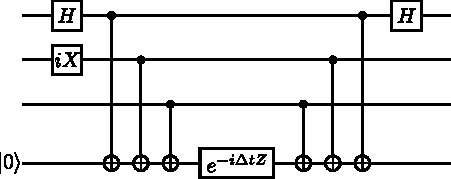
\includegraphics[scale=1.3]{figures/circuit_2.pdf}
\end{figure}
